\documentclass{article}
\usepackage[utf8]{inputenc}
\usepackage{graphicx}
\usepackage{hyperref}

\hypersetup{
    colorlinks=true,
    linkcolor=blue,
    filecolor=magenta,      
    urlcolor=cyan,
}

\title{\line(1,0){250}\\{\Huge \bigskip Gesture Consideration}\\\line(1,0){250}}
\author{ \footnotesize by \\[0.2cm] \footnotesize Gary Connelly (G00336837) \\[0.2cm] \footnotesize \& \\[0.2cm] \footnotesize Conor Raftery (G00274094)}
\date{\footnotesize April 2019}

\begin{document}

\maketitle
\bigskip
\bigskip
\bigskip
\bigskip
\bigskip
\bigskip
\bigskip
\bigskip
\bigskip
\bigskip
\bigskip
\bigskip

\includegraphics[width=\textwidth, height=150pt]{img/gmit-logo.jpg}
\clearpage

\tableofcontents
\clearpage

\section{Introduction}
This document looks at all of the considerations that were made by the development team when deciding what gestures to implement into this project. Originally, these considerations were going to be documented with the rest of the documentation, but it was eventually decided that this topic warranted a document of it's own. This document is broken down into five distinct sections including this introduction. The other four subsections are; "Gesture Research", in which any research conducted into what gestures would be used will be discussed, "Myo Armband Gestures \& Considerations", in which any gestures related to the myo armband, as well as the rational for their use will be discusses, "Speech Recognition Gesture \& Considerations", in which any gestures related to speech recognition, as well as the rational for their use will be discussed, and finally "Conclusion", in which the gestures as a collective will be discussed along with how well the team felt they worked. 

\clearpage

\section{Gesture Research}

\includegraphics[width=\textwidth, height=150pt]{img/Research.jpg}

\bigskip

Before considering what gestures were to be used, a research phase was undertaken by the development team. Topics that were looked at include instinctive gestures, gesture recognition, and the use of gestures. After careful consideration, the team narrowed down a list of each gesture and what possible actions each gesture would do.
\bigskip

After the gestures were decided upon, the team looked at what technologies would be incorporated into the project. This was followed closely by what each technology could do to enhance the project. The team looked at certain types games that could be created using the technology that was decided upon. This swayed the development team to creating a 2D Platform style game.
\bigskip

During the development of the project, a second research phase was completed. This research phase was conducted to discover possible solutions for navigating the Main Menu and Level Selection. The main gesture based technology that was studied was Speech Recognition. The team felt that Speech Recognition would add variety to the game, along with being extremely function-able.

\section{Myo Armband Gesture \& Considerations}
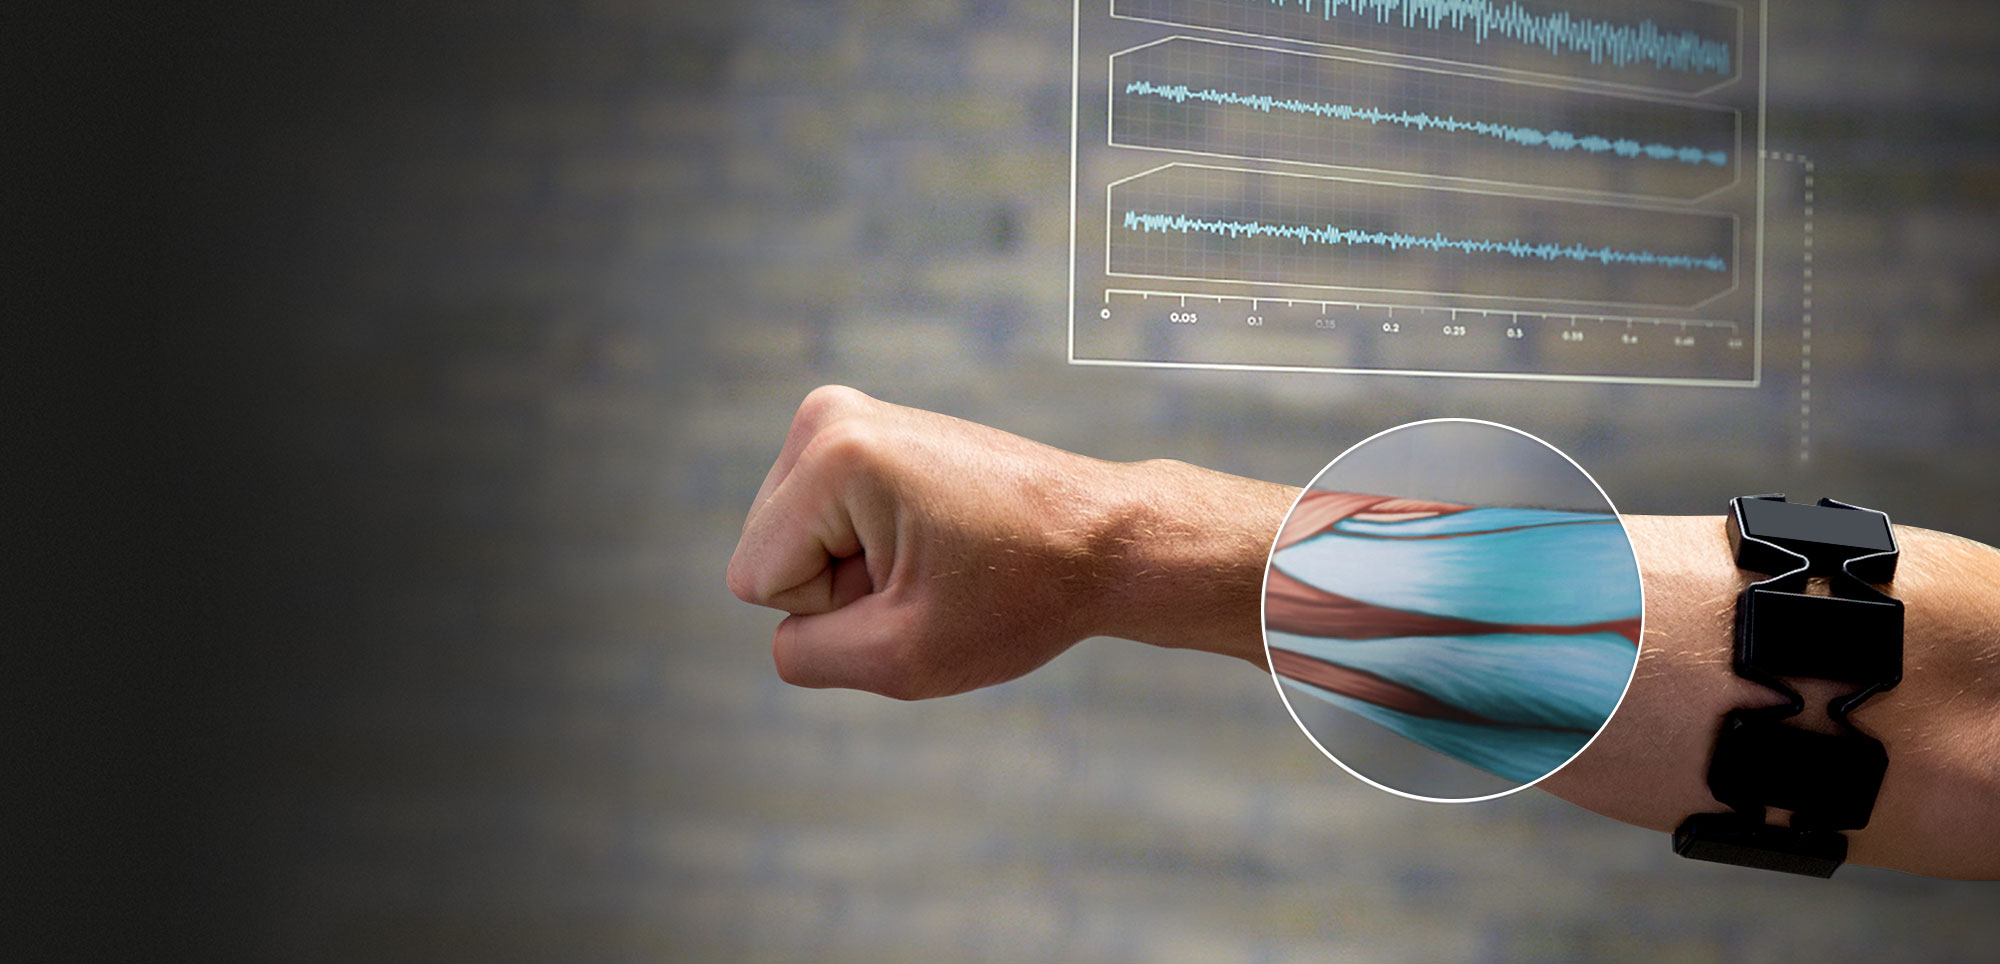
\includegraphics[width=\textwidth, height=150pt]{img/Myo.jpg}

\bigskip

In this section, the gestures relating to the myo armband will be discussed. The myo armband is able to recognise a whole host of gestures, including fingers spread, wave out, wave in, fist, directional up/down, and rotate.
\bigskip

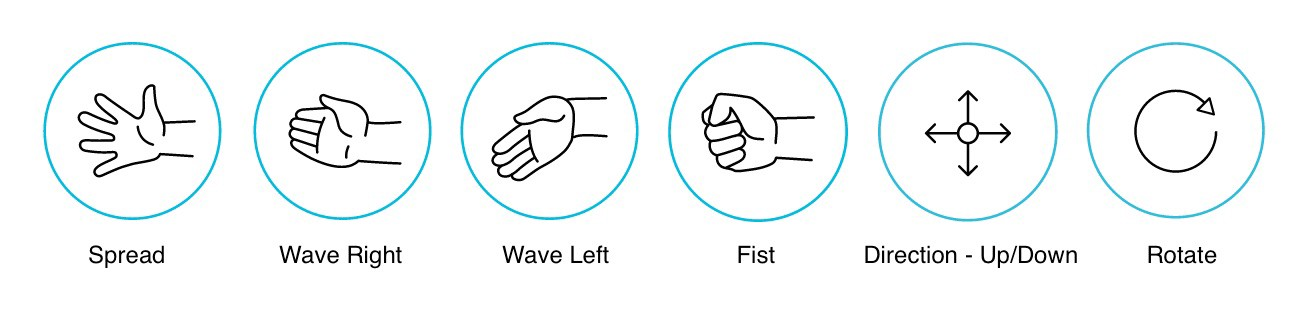
\includegraphics[width=\textwidth, height=100pt]{img/AllMyo.jpeg}

\bigskip

The gestures utilised in this application were wave out, wave in, and the fist gesture. These gestures will be discussed in more detail in the next few sub-sections.

\subsection{Actions}
The gestures that were chosen to be implemented into this project were selected based upon what actions the game character needed to be able to do in the game. The development team wanted the gestures to be as intuitive and simple to use as possible. The main actions the game character needed to be able to do in the game were, move left, move right, and shoot. 



\subsubsection{Move Left}

The first actions that had to be considered were the actions that make the game character move. In this particular game, the game character need only move left and right along the X-axis. There is no vertical movement needed at all. 

With this in mind, it made sense to the development team, to map the wave in and wave out gestures to the game characters left and right movements.

\bigskip

Due to the fact that most people are right-handed, the majority of people will automatically put the myo armband onto their right arm. With the myo in their right arm, when they make a wave-in gesture, their hand will be pointing to the left. Therefore, it made the most logical action to map to this gesture would be to move the player to the left.


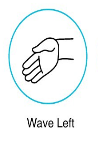
\includegraphics[width=100pt, height=100pt]{img/WaveLeft.PNG}

\bigskip

\subsubsection{Move Right}

The same logic applies to map a gesture to the action of making the player move right. When a majority of people put the myo armband on their right arm by default, when they wave out, their hand will be pointing it the right. As for the minority of people who will automatically put the armband on their left arm, a tutorial will need to be shown in a scene in the game to let the user know that the myo should be on their right arm.  

\bigskip

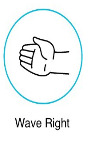
\includegraphics[width=100pt, height=100pt]{img/WaveRight.PNG}

\bigskip

\clearpage

\subsubsection{Shoot}
In the game itself, the game character must try to pop bubbles by shooting a hook upwards at them. The gesture that was selected to perform this action was the fist gesture.

\bigskip

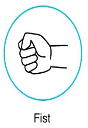
\includegraphics[width=100pt, height=100pt]{img/Fist.PNG}

\bigskip

Initially, the development team found it difficult to pick between using the fist gesture, and the double-tap gesture. This was because of the fact that both team members felt that both gestures could fit quite well with a shooting action. 
To break the tie, the team ended up simply testing both gestures to determine which one worked better. This test supplied the team with enough knowledge to make an informed decision. 

\bigskip

The team felt that the  fist gesture was the better option of the two for two reasons; the first reason being that they felt it was a more natural movement to go from waving ones hand from side to side, to making a fist. The motion simply felt cleaner as opposed to the motion of goring from moving ones hand from side to side, to then doing a double-tap gesture.
The second reason the team felt the would be quicker.

\subsubsection{Unused Gestures}
There were many myo gestures that the development team wanted to integrate into the application, but they unfortunately could not come up with a creative way of doing so without compromising the users experience.

Two main gestures that the development team wanted to add were the fingers spread gesture, and the double tap gesture.

\bigskip

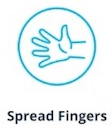
\includegraphics[width=100pt, height=100pt]{img/Spread.PNG}
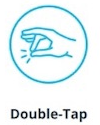
\includegraphics[width=100pt, height=100pt]{img/DoubleTap.PNG}

\bigskip

The reason the team wanted to implement these gestures, was because of the fact that they wanted to express the full functionality of the technology that was available to them. The plan was to integrate these gestures into an in-game pause menu that the user could interact with using only myo gestures. However, when it came to testing this, certain issues were encountered. The most common issue was the pause menu popping up and pausing the game without it being the users intentions. This is could be due to the fact that as the player is playing a game like this, they may be inclined to tense up their arm if they are under pressure. If they do this, the myo may get inaccurate readings causing the pause menu to spawn seemingly out of no where. 

\bigskip

In the best interests of the end user, the development team thought it best to have a strict gestural divide between game play and navigation, hence the speech recognition navigation system.



\subsection{Conclusion}
The development team were very happy with how the myo gestures work with the game. For the most part, there is a seamless interaction between the myo armband and the game character. There are certain occasions where the communication breaks down between the myo armband and the app however. For example, if the user has an old device that is running quite slow, or if the myo armband itself is worn out or damaged, the interaction might suffer latency issues. This issue is exaggerated by the fact that the whole point of the game is to have quick reactions or the player dies. 

Another potential issue that has been noted has less to do with the technology, and more to do with the nature of the game itself. This is especially the case in the later levels of the game. Whenever a user is rapidly trying to avoid multiplying bubbles bouncing around the screen, the first thing the user does is tense up their arm. As mentioned before, this tension can cause inaccuracies in the communication between the myo armband and the game character. 

\section{Speech Recognition Gesture \& Considerations}
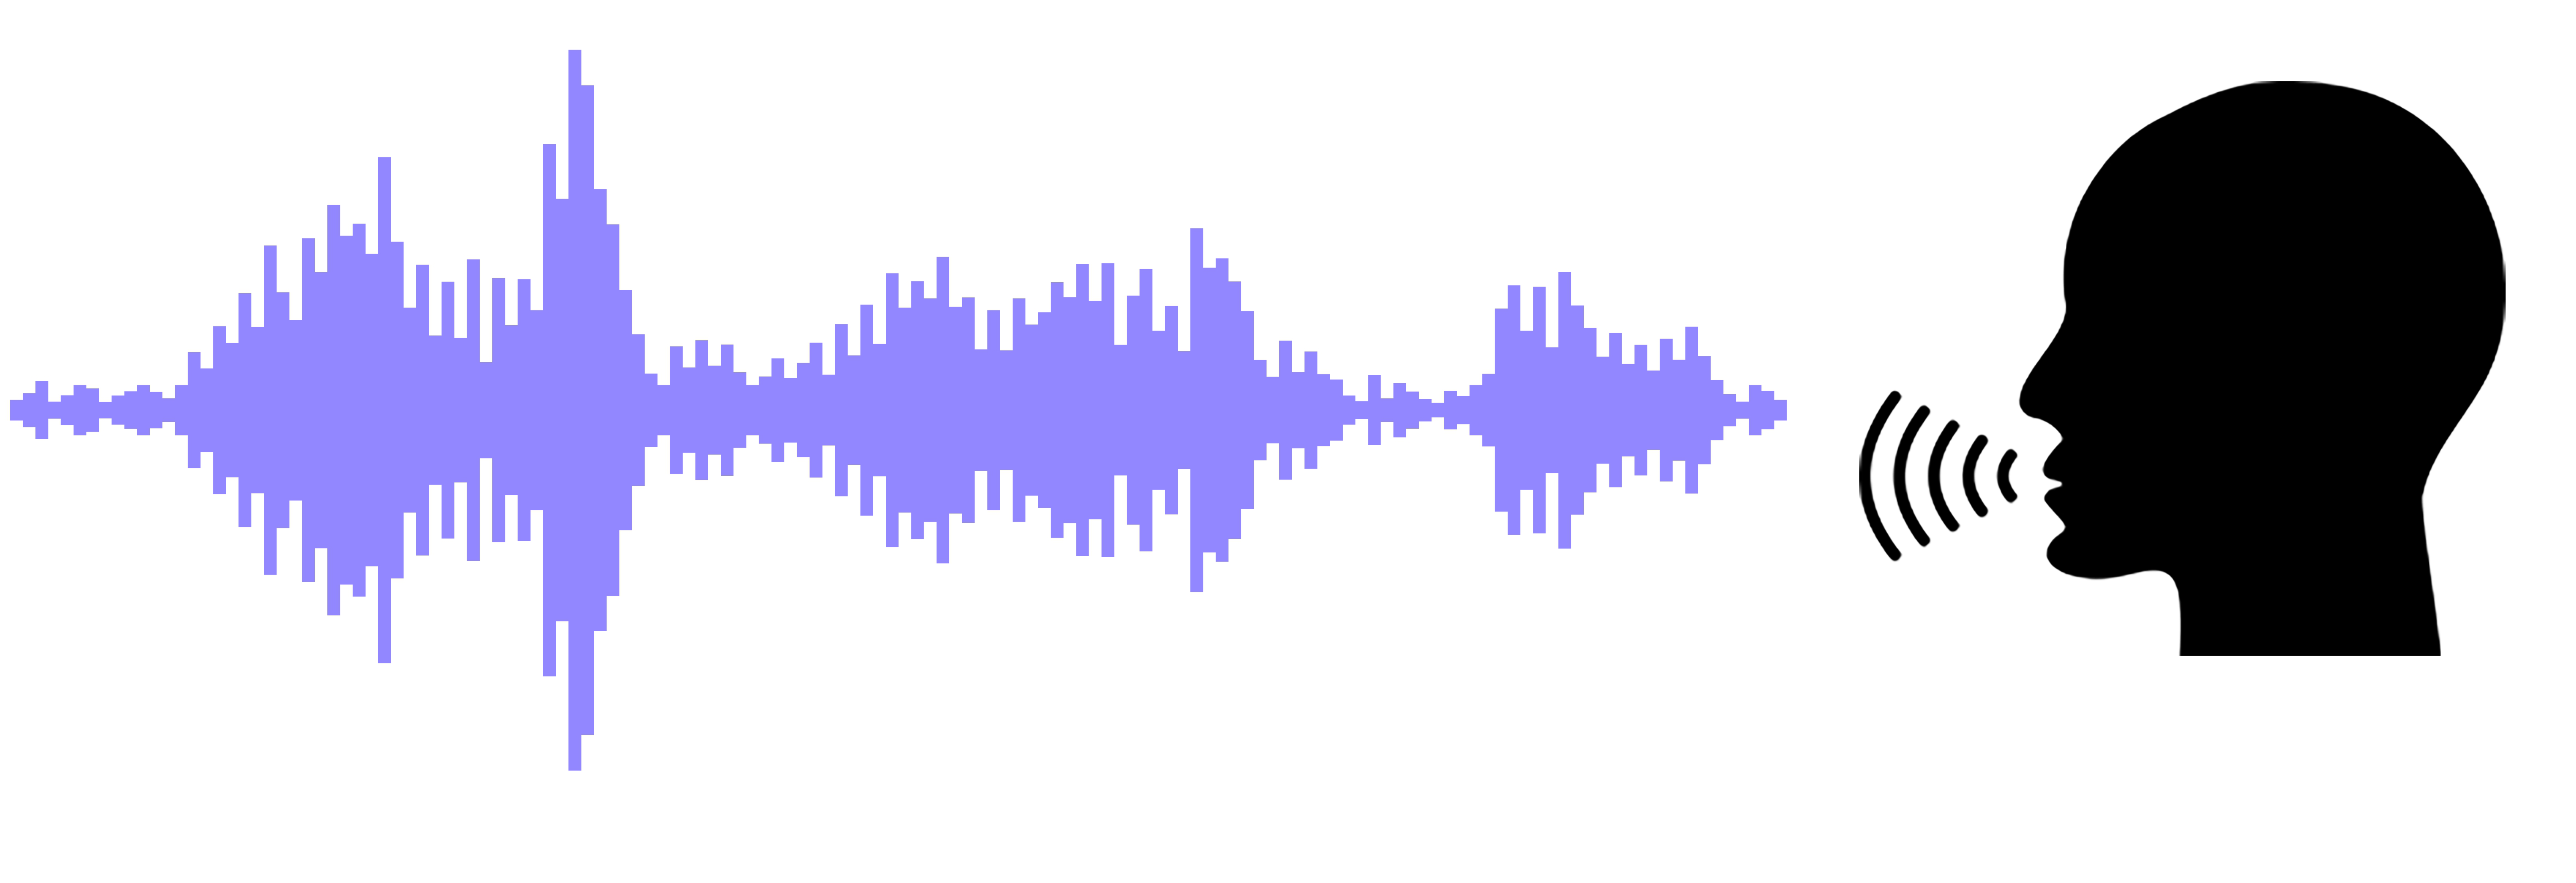
\includegraphics[width=\textwidth, height=100pt]{img/speechrecognition.png}
\bigskip

Consideration for speech recognition was done late into the projects development. It was decided that the project needed more variety in terms of gesture UI. The team wanted to remove all keyboard and mouse input in the project. This was to fully submerse the game with gesture controls.
The speech recognition was incorporated into the project by using Unity's keyword recognizer. This is achieved by importing 'UnityEngine.Windows.Speech'. This allows the user to use their personal microphone which is built into the device the game is being played on. This must be enabled before use. The speech recognition is able to detect a letter, a word and even a phrase.

\subsection{Menu Navigation}
The speech recognition is used purely in the functional end of the project. These being the subheadings below. The team decided against using the speech recognition for the in-game play as it was determined too slow for the quick reactions needed during gameplay.

\subsubsection{Main Menu Navigation}
The Main Menu was the first area where the speech recognition was implemented. The main menu is the initial scene that is loaded when the project is ran. This scene contains a panel within a canvas, and withing this panel, are two buttons. A 'Play Game' button and a 'Quit' button.

\bigskip

These buttons are accessed via the speech recognition technology. The 'Quit' button is activated by either speaking 'Quit', or 'Exit'. When the button is activated, the game will quit by displaying 'quit' to the console.

\bigskip

The 'Play' button is triggered by speaking either 'Start' or 'Quit'. This button is used to load the next scene. The rational behind using multiple trigger words (or phrases) was to add to the robustness of the game. The scene that will be loaded when the 'Play' button is triggered is the Levels Menu.

\subsubsection{Levels Menu Navigation}
This menu is similar to the Main Menu, as it has multiple buttons contained within a canvas \& panel. These buttons are triggers to load each of the game levels. The development team decided to add a 'return to main menu' option. This is activated by the user speaking the word(s) 'Main Menu', 'Back' or 'Return'.

\bigskip

Each level button has multiple keywords attached that are recognized by the speech recognition technology. When one of the these keywords are triggered, the relevant level (scene) is loaded. These keywords are:
\begin{itemize}
  \item Level 1: 'Level One' or 'One'
  \item Level 2: 'Level Two' or 'Two'
  \item Level 3: 'Level Three' or 'Three'
  \item Level 4: 'Level Four' or 'Four'
  \item Level 5: 'Level Five' or 'Five'
\end{itemize}
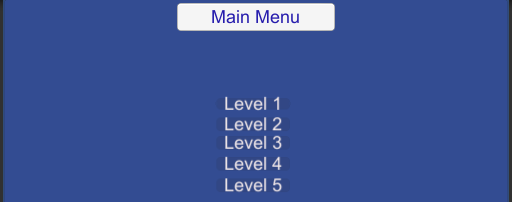
\includegraphics[height=100pt]{img/levelsMenu.PNG}


\subsubsection{In-Game User Interaction}
The final section where the speech recognition is used is during the in-game play. The team took consideration that the user would need to be able to pause the game when the moment arises. This was initially going to be controlled by a Myo Armband gesture execution, but there was a major flaw to this decision. The user could accidentally pause the game due to the inaccuracy of the Myo Armband. This led to the decision to use speech recognition for this function.

\bigskip

The voice command for pausing the game (during gameplay) is 'Pause'. This will 'freeze' the game and stop the time until the user gestures the word 'Resume'. When this word his executed, the game will continue. While in the Pause Menu, the user will also have to option to return to the Levels Menu by speaking the word 'Main Menu'.

\subsection{Conclusion}
The team found the speech recognition was considerably easy to configure and to implement into the project. It adds a lot of variation to the project by including multiple gestures in which to control the program. The keyword recognizer is quite flexible as you can apply multiple keywords and phrases to the same function. This also adds robustness to the program. The team concludes that the speech recognition is a vital part to the project for the reasons suggested above.

\clearpage

\section{Conclusion of Gesture Rational}

Although the development team were quite happy with how the gestures integrate seamlessly, there are certain aspects that would be reconsidered. If this project was to be redone, more time would be put into considering the inclusion of the outlying Myo gestures, along with adapting the speech recognition technology to other areas of the project. For example, the use of the finer tap and finger spread. The development team considered providing the option of using the menu control system with the Myo Armband, as this might be a preferred interaction for some users, especially if they are using the game within a public space. 

\end{document}
